\documentclass{beamer}
\usepackage{transparent}
\usepackage[beamer]{shortcuts_tom}


\usepackage[autoplay]{animate}
\usepackage{bibentry}
\usepackage{subcaption}
\usepackage{appendixnumberbeamer}

\graphicspath{{./images/}}
\def\TikzLocation{./tikz/}
\def\tkzscl{1}
\definecolor{linkcolor}{RGB}{83,83,182}


%\setbeamercolor{block title}{fg=darkred}
%\newcommand{\btitle}[1]{{\usebeamerfont{block title}\usebeamercolor[fg]{block title} #1}}

\AtBeginSection[]
{
}


\makeatletter
\def\beamer@newblock{%
  \usebeamercolor[fg]{bibliography entry author}%
  \usebeamerfont{bibliography entry author}%
  \usebeamertemplate{bibliography entry author}%
  \def\newblock{%
    \usebeamercolor[fg]{bibliography entry title}%
    \usebeamerfont{bibliography entry title}%
    \usebeamertemplate{bibliography entry title}%
    \def\newblock{%
      \usebeamercolor[fg]{bibliography entry location}%
      \usebeamerfont{bibliography entry location}%
      \usebeamertemplate{bibliography entry location}%
      \def\newblock{%
        \usebeamercolor[fg]{bibliography entry note}%
        \usebeamerfont{bibliography entry note}%
        \usebeamertemplate{bibliography entry note}}}}%
  \leavevmode\setbox\beamer@tempbox=\hbox{}\ht\beamer@tempbox=0em\box\beamer@tempbox}
  \setbeamertemplate{bibliography entry title}{}{}

\makeatother

\usepackage[square, authoryear]{natbib}


%-----------------------------------------------------------------------------
%	CUSTOM COMANDS
%-----------------------------------------------------------------------------

\def\keypoint#1{\hspace{0pt plus 1 filll}\textcolor{gray}{[{\color{linkcolor}#1}]}~}
\def\mycite#1{\keypoint{\small\citep{#1}}}
\def\citeconf#1#2{
    {\textcolor{gray}[}%
        {\color{linkcolor}\citealt{#1}, #2}%
    {\textcolor{gray}]}}
\def\citeconfright#1#2{\hspace{0pt plus 1 filll}{\small\citeconf{#1}{#2}~}}
\def\biblio{
	\nobibliography{library}
	\def\biblio{}
}

\def\myitem{\hskip1ex{\color{linkcolor} $\blacktriangleright$}\hskip.3em}



\newcommand{\overimg}[4]{
    \begin{tikzpicture}
    \only<#1-#3>{%
        \node {\includegraphics[height=.6\textheight]{#2}};
    }%
    \only<#3>{%
        \node {\includegraphics[height=.5\textheight]{#4}};
    }%
    \end{tikzpicture}
}


%\usepackage{lxfonts}

\institute{INRIA Saclay ~~ -- ~~ MIND}
\author{Thomas Moreau}
\title{ML/AI for Physical signals}


\setbeamertemplate{title page}[frame]


\begin{document}

\begin{frame}[plain]
\titlepage
\biblio{}
\end{frame}

\def\biblio{}


\frame{
    \frametitle{Biophysical systems}

    \definecolor{Z}{RGB}{45,162,65}
    \definecolor{D}{RGB}{180,35,35}
    \def\varX{{\color{linkcolor} \pmb X}}
    \def\varZ{{\color{Z} \pmb \varepsilon}}
    \def\varD{{\color{D} \pmb G}}
    {\centering
    \begin{tikzpicture}
    \tikzset{
        %Define standard arrow tip
        >=stealth',
        %Define style for boxes
        varstyle/.style={
            rectangle,
            rounded corners,
            draw=black,
            text width=1em,
            minimum height=1.5em,
            text centered},
    }
    \node (meg) {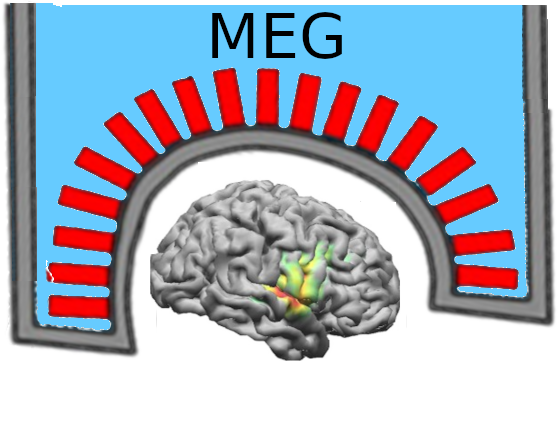
\includegraphics[width=12em]{meg_localised_source}};
    \draw[->, thick] ($(meg.east) - (0, 1.5em)$) -- ++(8em, 0)
    node[midway, align=center] (maxwell) {Maxwell's\\Equations}
    node[right] (topomap) {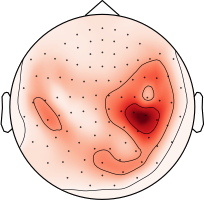
\includegraphics[width=6em]{topomap_somato}};
    \node[varstyle, below=.5em] at (topomap.south) (varX) {$\varX$};
    \node[below=0em of varX.south] {\bf Observed signal};
%        \draw[->, thick] (topomap.east) -- ++(5em, 0)
%        node[midway, align=center] {\small Problème\\ \small inverse}
    \node[varstyle, below=.2em of meg]
        (varZ) {$\varZ$};
        \node[below=0em of varZ.south] {\bf Electrical activity};
    \node[varstyle, below=3.8em of maxwell.center]
        (varD) {$\varD$};

    \uncover<2->{
         \draw[<-, thick] (meg.east) to[bend left, looseness=1]
            node [midway, above] {Inverse Problem}
            ($(topomap.west) + (0, 1.5em)$);
    }
    \end{tikzpicture}}
    \vskip0em
    {\bf Forward model: }$\varX{} = \varD\varZ$
    \hskip3em
    \uncover<2->{{\bf Inverse problem:} $\varZ = f(\varX)$ (ill-posed)}\\[1em]
    \uncover<3->{\centering
        \myitem{} Dipole fit
        \hskip2em
        \myitem{} Regularized optimization
        \hskip2em
        \myitem{} Deep-learning\\
        \mycite{Sarvas1987}\hskip2em
        \mycite{Gramfort2012}\hskip2em
        \mycite{Hecker2021}
    }

}


\frame[c]{

    \frametitle{Event based signal processing}

    \centering
    \only<1-2>{
        \begin{itemize}
            \item Quantification de l'équilibre dynamique.\\[1em]
        \end{itemize}
        \overimg{1}{applications/accelero}{2}{applications/accelero_dict}

        \textcolor{gray}{[{\color{linkcolor} PLoS ONE 2016; Sensors 2018}]}\\
    }
    \only<3-4>{
        \begin{itemize}
            \item Caractérisation de mouvements oculaires pathologiques.\\[1em]
        \end{itemize}
        \overimg{3}{applications/oculo}{4}{applications/oculo_dict}

        \textcolor{gray}{[{\color{linkcolor} EMBC 2020}]}\\
    }
    \only<5-6>{
        \begin{itemize}
            \item Comptage d'objet astronomiques dans des images de telescope.\\[1em]
        \end{itemize}
        \overimg{5}{applications/Hubble}{6}{applications/Hubble_dict}

        {\centering\textcolor{gray}{[{\color{linkcolor}TPAMI 2020}]}\\}
    }
    \only<7-8>{
        \begin{itemize}
            \item Exploration des signaux neurologiques de l'ECG, la MEG ou l'IRMf.\\[1em]
        \end{itemize}
        \overimg{7}{applications/meg_1}{8}{applications/meg_dict}

        \textcolor{gray}{[{\color{linkcolor} NeurIPS 2018; ICASSP 2019}]}\\
    }

}

\frame{
    \frametitle{Challenges}

    \begin{itemize}
        \item Large amount of data
        \item Cannot have all the data on one node.
        \item Type of algo
        \begin{itemize}
            \item Anomaly detection,
            \item Pattern Analysis
        \end{itemize}
        Not completely the scope of sklearn (signals)
    \end{itemize}
}

\frame{
    \frametitle{Scikit-Learn out-of-core API}

    For now: \texttt{partial\_fit}\\[2em]

    How to do some out of core:\\
    \begin{itemize}
        \item Efficient distributed datastructure (dask? Other?)\\
        \item Distributed training
    \end{itemize}


}

\frame{
    \frametitle{Joblib: Pluggable backend for sklearn}

    \begin{itemize}
        \item Simple library for embarassingly parallel workflow
        \item Pluggable backend -- easy to move from sequential, to threads, processes and distributed.
        \item On disk caching for fault resilience.
    \end{itemize}

}

\frame{
    \frametitle{Distributed Optimization}


}


\end{document}
